\chapter{DESIGN}

\noindent{We design an efficient  scheme to generate certificates for users to prevent certificate forgery. 
In our proposed scheme, only authorized parties have permission to generate certificates 
The scheme verifies the authenticity and genuineness of certificates. 
We used a decentralized storage system to avoid no single point of failure(IPFS).
}

\section{DATAFLOW DIAGRAM}
\begin{figure}[H]
    \centering
    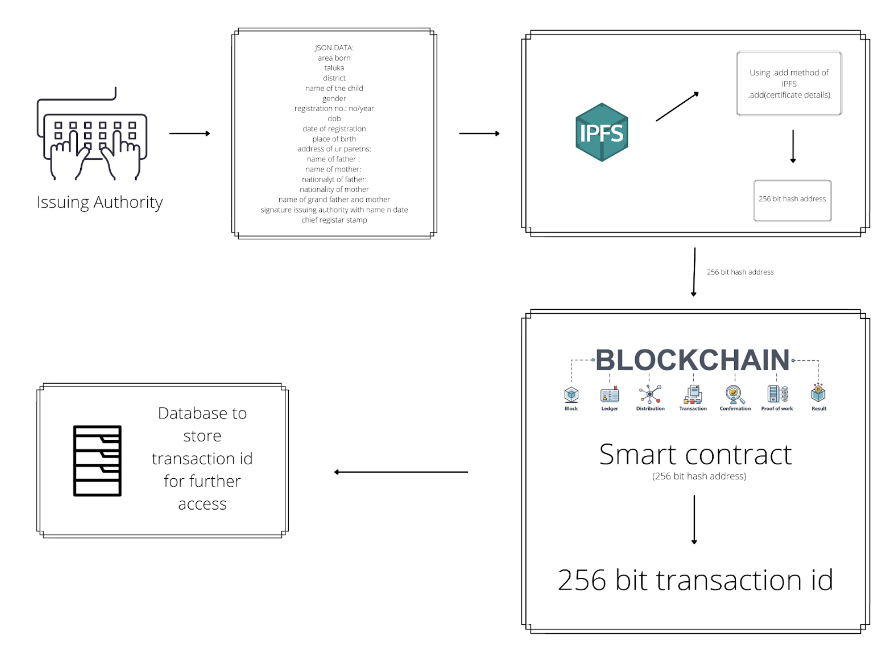
\includegraphics[width=.90\textwidth]{imgs/dataflow_diagram.png}
    \caption{Dataflow diagram of the project}
    \label{fig:Dataflow diagram of the project}
    \end{figure}

\section{BLOCK DIAGRAM}
\begin{figure}[H]
    \centering
    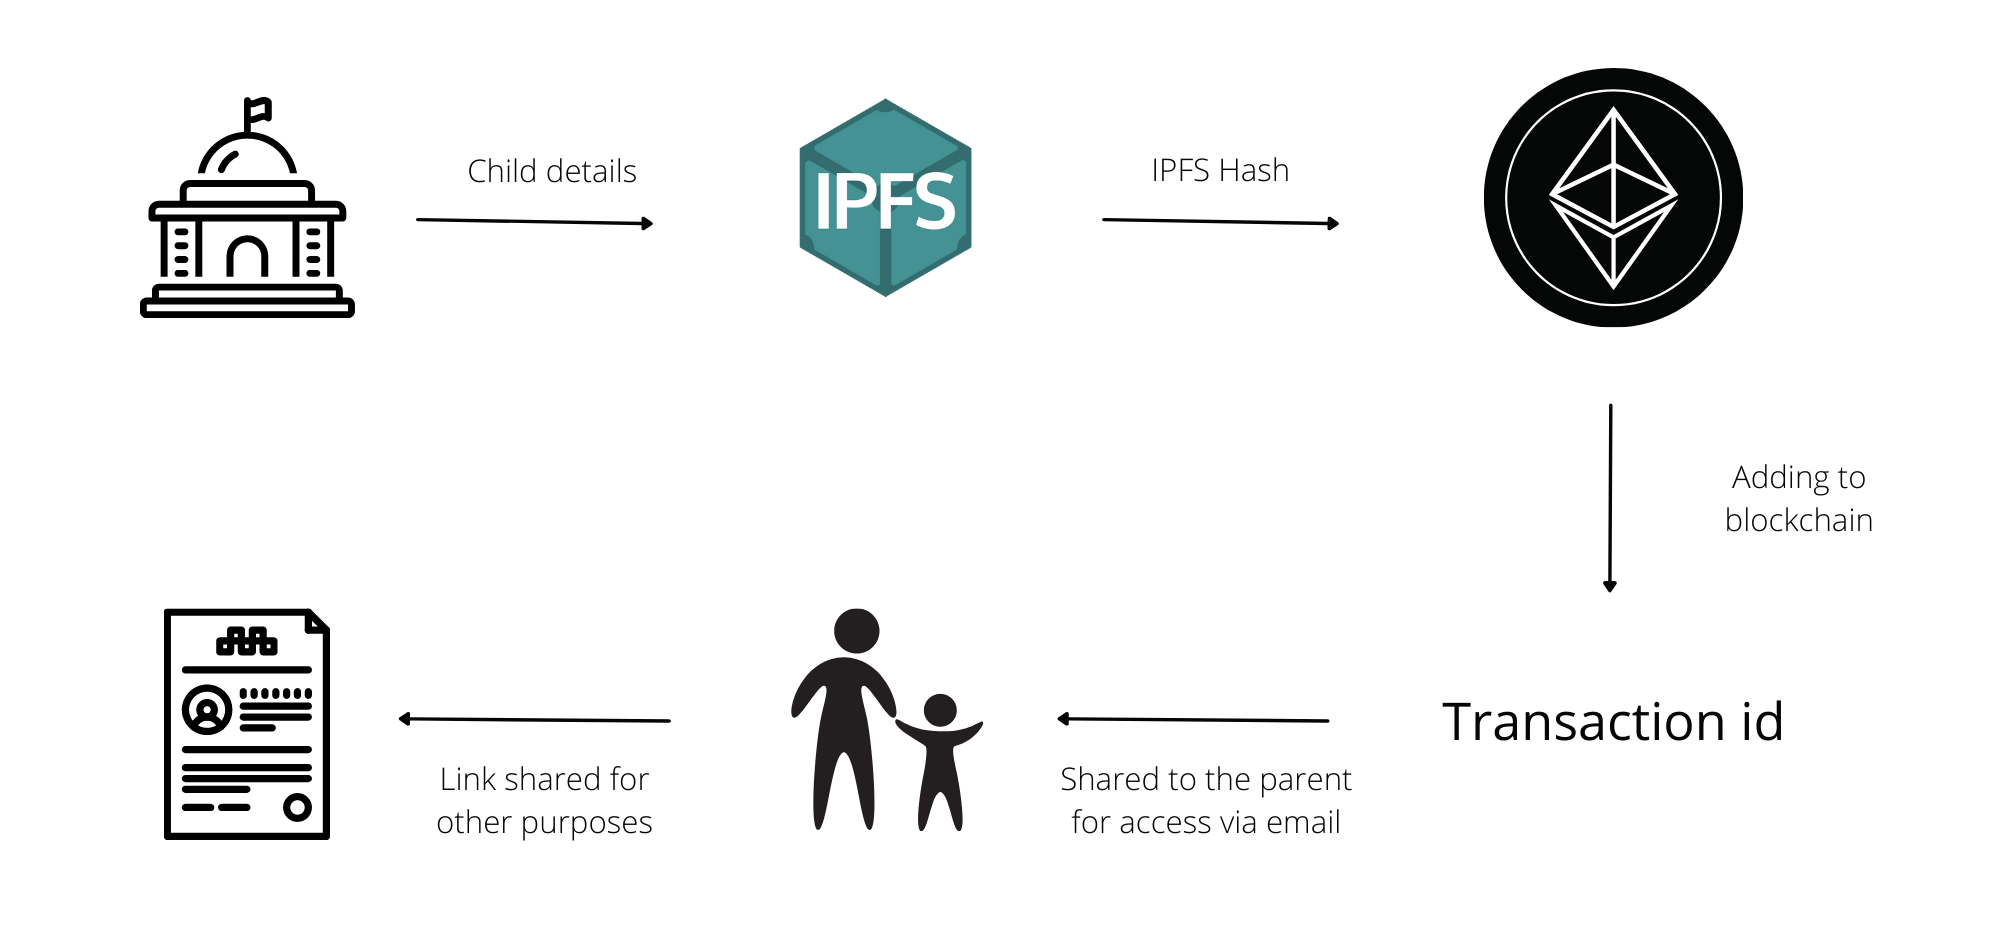
\includegraphics[width=\textwidth]{imgs/Basic_working.png}
    \caption{Block diagram of the project}
    \label{fig:Block diagram of the project}
    \end{figure}

\vspace{1cm}

    \section{USECASE DIAGRAM}
    \begin{figure}[H]
        \centering
        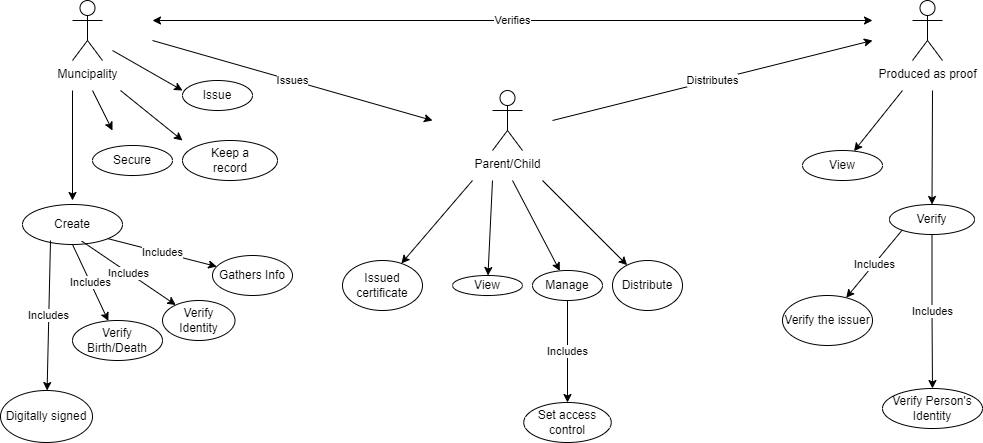
\includegraphics[width=\textwidth]{imgs/Use_case_diagram.png}
        \caption{Usecase diagram of the project}
        \label{fig:Usecase diagram of the project}
        \end{figure}
    

    \section{EXTERNAL FLOW DIAGRAM}
\begin{figure}[H]
    \centering
    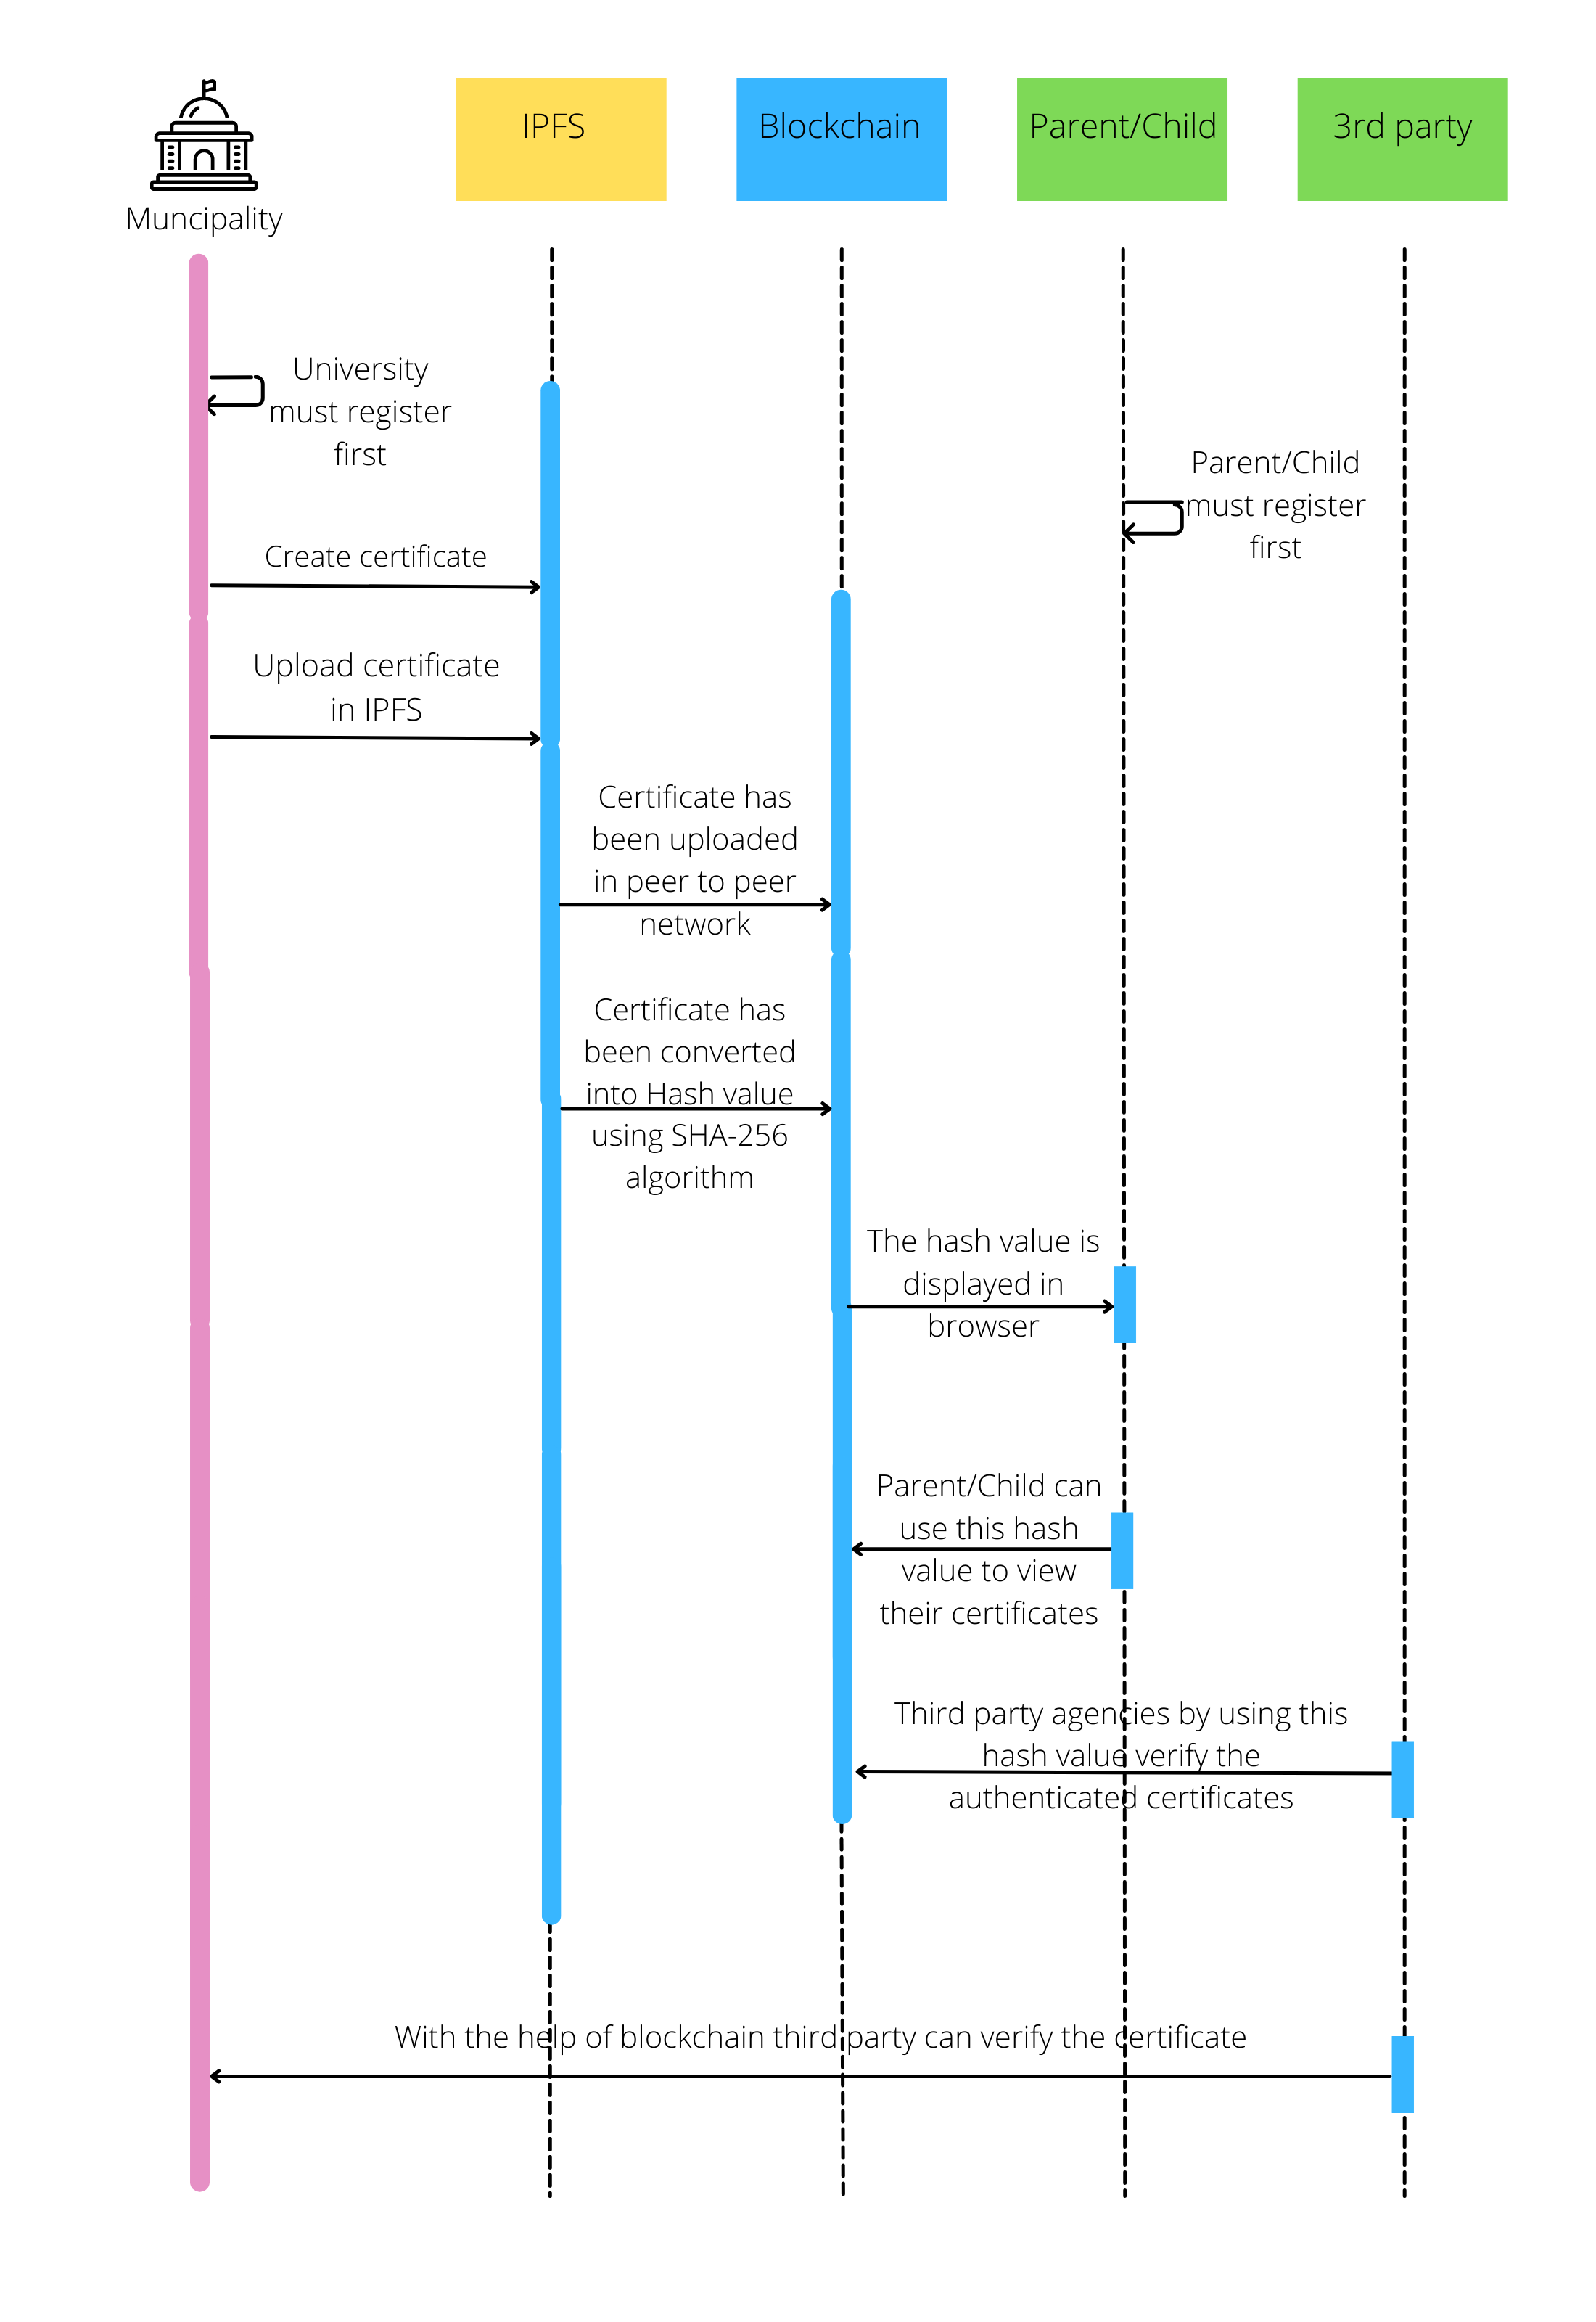
\includegraphics[width=0.80\textwidth]{imgs/External_flow.png}
    \caption{External flow diagram of the project}
    \label{fig:External flow diagram of the project}
    \end{figure}
